\chapter{Zero-Touch External Hardware Transfer on a \texorpdfstring{\SI{24.2}{\giga\hertz}}{24.2 GHz} Neonatal Thorax Simulator}
\label{ch:external_transfer}

\section{Purpose and scope}

Chapter~5 examined selective uncertainty and finite-sample conformal calibration within the neonatal intensive-care-unit (NICU) reconstruction. This chapter asks a different question: do the frozen estimators retain their respiratory-rate tracking behavior when the radar hardware and signal source change? Stage~4 addresses this question with an independent 24.2~GHz radar recording of a controlled neonatal thorax simulator and a synchronized laser micrometer reference. The public dataset contains programmed sinusoidal breathing at ten rates from 5 to 80 breaths per minute (bpm), each in normal and deep excursion modes \citep{gleichauf2024time}.

This is a zero-touch hardware-transfer benchmark, not an external patient cohort. It tests whether models frozen after the NICU experiments can recover a known periodic mechanical signal on a different radar device, under a different acquisition chain, without external-data tuning. Its value is that the signal and reference are controlled and the hardware differs from the training system. Its limit is equally important: a simulator does not reproduce the variability, irregular breathing, motion, and clinical events found in infants. Results below support the bounded claim of transfer to these stationary simulator scenarios; they do not establish patient-level generalization, clinical accuracy, or bedside utility.

\section{External benchmark protocol}
\label{sec:ch6_protocol}

\subsection{Dataset, reference, and domain shift}

The external recordings are from the Gleichauf et al. neonatal thorax simulator dataset. A 24.2~GHz continuous-wave radar (InnoSenT iSYS-4001) records the simulated chest motion, while an approximately 2.5~kHz laser micrometer provides the independent displacement reference. The NICU system used in the earlier chapters operated at 24.0~GHz and 16~Hz. External radar I/Q data were acquired at approximately 2~kHz and deterministically decimated to the locked 16~Hz model input. Thus the transfer changes the radar unit and acquisition rate while retaining the frozen estimation pipeline and the independent physical reference.

The radar signal was mean-centered and passed through the locked zero-phase Kaiser FIR bandpass filter with $\firTaps=64$ taps, passband $[\bandLow,\bandHigh]=[0.30,3.00]$~Hz (18--180~bpm), and $\kaiserBeta=6.5$. The estimator's respiratory-rate grid is 18--90~bpm. Thus, 20~bpm lies within the grid but near the filter's lower transition skirt, whereas 5 and 10~bpm lie below both the passband and the estimator grid. The downsampling used two polyphase stages, first to approximately 200~Hz and then to 16~Hz; the resampling gain variation across the tested rates remained between $-0.0003$ and $+0.0023$~dB. The laser-derived steady-state rate was recomputed from the reference signal and used as the evaluation ground truth (matching the programmed rates within 0.036~bpm across all 20 scenarios). No model parameter, threshold, filter, window, scaler, or calibration quantile was adjusted using the external recordings.

The primary point estimate uses the full-cohort $K=11$ parameterization loaded from the frozen Stage~3 model archive. The archive's SHA-256 digest is \texttt{af33a83e\allowbreak 157f7d2e\allowbreak fb0f47e5\allowbreak 0c9544ee\allowbreak 19bacb7d\allowbreak a88ab0e0\allowbreak 235ccead\allowbreak 029cbcc4}. A leave-one-patient-out mean parameterization is reported as a sensitivity analysis; it was also transferred without external adaptation. The archive was frozen before this benchmark, and external data were used only for the one-shot evaluation.

\subsection{Scenario partition and evaluation window}

There are 20 programmed scenarios: rates of 5, 10, 20, 30, 40, 45, 50, 55, 60, and 80~bpm, each in normal and deep mode. For the Stage~4 report, scenarios were partitioned before scoring into an in-band set at or above 28~bpm and a sub-band set below 28~bpm. The resulting 14+6 partition is exhaustive (Table~\ref{tab:ch6_scenario_partition}). The 28~bpm boundary separates the primary operating region from the lower-frequency transition skirt and stopband; it is an operational reporting boundary, not a tested rate, since the nearest programmed conditions are 20 and 30~bpm. The analysis plan stated qualitative transfer goals, while the numeric thresholds in Gate~G5 are audit operationalizations rather than clinical decision thresholds.

\begin{table}[htbp]
\centering
\footnotesize
\caption{Exhaustive Stage~4 scenario partition. Each programmed rate was recorded in normal and deep excursion modes.}
\label{tab:ch6_scenario_partition}
\begin{tabularx}{\textwidth}{@{}>{\raggedright\arraybackslash}p{4.6cm}>{\raggedright\arraybackslash}Xr@{}}
\toprule
Stratum & Programmed rates & Scenarios \\
\midrule
In-band ($\brRef\geq28$~bpm) & 30, 40, 45, 50, 55, 60, 80~bpm & 14 \\
20~bpm FIR transition skirt & 20~bpm & 2 \\
05--10~bpm below-grid stopband & 5, 10~bpm & 4 \\
Sub-band total ($\brRef<28$~bpm) & 5, 10, 20~bpm & 6 \\
All scenarios & 5--80~bpm, ten programmed rates & 20 \\
\bottomrule
\end{tabularx}
\end{table}

The primary tracking metrics use overlapping 30~s windows advanced in 2~s steps, matching the prior stages, and retain steady-state windows only. Windows beginning before 10~s or ending within 10~s of the recording end were excluded, removing start and end synchronization steps. A separate all-window tracking sensitivity regime includes those transients, whereas the Stage~4 uncertainty risk--coverage audit evaluates steady-state windows and isolates the excluded start/end transients in a dedicated transient-detection check. In-band performance is summarized both as a scenario-macro mean, which weights the 14 conditions equally, and as a pooled-window metric. These summaries answer different questions and are not interchangeable. In total, the primary in-band evaluation contains 6,049 windows; the 5--10~bpm stopband comparison contains 1,731 windows.

\section{Zero-touch respiratory-rate transfer}
\label{sec:ch6_tracking}

\subsection{In-band accuracy and model complexity}

Within the 14 in-band conditions, the physics-constrained R0--R2 models track the simulator's stable periodic motion with very low scenario-macro error (Table~\ref{tab:ch6_model_transfer}). The primary frozen model, R2e, has a scenario-macro RMSE of 0.0197~bpm and a pooled-window $\rmsePool$ of 0.0262~bpm; its scenario-macro MAE is 0.0184~bpm. It achieves $\accTau{3}=\accTau{6}=\accTau{10}=100\%$, a calibration slope of 0.9994, and Pearson correlation $r=0.999999$ across scenario means. No steady-state R2e estimate differs from the laser reference by more than 0.5~bpm; its largest absolute error is 0.158~bpm. The LOPO-mean sensitivity gives a scenario-macro RMSE of 0.023~bpm, close to the full-cohort result.

R2e is the designated primary model because it is the frozen eight-parameter causal estimator carried forward from Stage~3, not because it wins every simulator point estimate. The 11-parameter R2a has a slightly lower scenario-macro RMSE (0.0189~bpm), and the offline R1f smoother is lower still (0.015~bpm) but is not a real-time comparator. R0 and the three-parameter causal R1a are also around 0.03~bpm. On this controlled in-band signal, adding parameters within the constrained family produces only tiny absolute differences.

\begin{table}[htbp]
\centering
\footnotesize
\setlength{\tabcolsep}{4pt}
\caption{Stage~4 steady-state tracking by model on the 14 in-band scenarios. RMSE, MAE, and bias are scenario-macro means in bpm; the 80~bpm and 20~bpm columns give RMSE for those two-scenario strata. R1f is an offline reference.}
\label{tab:ch6_model_transfer}
\begin{tabularx}{\textwidth}{@{}>{\raggedright\arraybackslash}Xrrrrrr@{}}
\toprule
Model & Params & RMSE & MAE & Bias & 80~bpm & 20~bpm \\
\midrule
R0 physical baseline & 0 & 0.028 & 0.027 & $-0.005$ & 0.063 & 0.069 \\
R1a causal forward estimator & 3 & 0.030 & 0.028 & $-0.007$ & 0.011 & 0.161 \\
R1f offline smoother & 3 & 0.015 & 0.014 & $+0.001$ & 0.010 & 0.053 \\
R2e causal, primary & 8 & 0.020 & 0.018 & $+0.001$ & 0.009 & 0.095 \\
R2a causal, 11-parameter & 11 & 0.019 & 0.017 & $+0.003$ & 0.020 & 0.024 \\
R3c spectral ridge & 439 & 3.635 & 3.607 & $+0.618$ & 10.465 & 11.778 \\
R3b spectral MLP & 14.6k & 3.502 & 3.447 & $+3.402$ & 1.065 & 32.704 \\
R3a causal TCN & 15.8k & 3.178 & 3.127 & $+0.695$ & 7.533 & 23.471 \\
\bottomrule
\end{tabularx}
\end{table}

The unconstrained rung-3 models show a different pattern. Their in-band scenario RMSEs range from 3.18 to 3.64~bpm, despite high scenario-level Pearson correlations (0.967--0.991). Correlation alone therefore hides errors in calibration and rate-dependent tracking: R3c has slope 0.709 and underestimates the 80~bpm condition, while R3b has a +3.402~bpm mean bias. Training sizes also differ: R3c and the R2 models were fit using all 11 NICU infants; R3a and R3b used 10, with one infant held out for early-stopping selection. This disclosure matters when interpreting the comparison, although all models were evaluated on the same independent simulator scenarios.

These findings support a limited inference: on the stable in-band simulator waveforms, the constrained signal-processing and state-space estimators transfer more reliably than the tested learned shortcuts. They do not show that a given model is more accurate on infants, where the reference modality, noise profile, and physiological variability differ from this controlled comparison.

\subsection{Rate-by-rate behavior and the filter boundary}

Table~\ref{tab:ch6_rate_by_rate} reports R2e for all 20 conditions, and Figure~\ref{fig:ch6_frequency_transfer} compares rate transfer and passband error across model rungs. Each cell gives scenario RMSE followed by the mean estimated rate in parentheses. From 30 through 80~bpm, the model follows the laser reference closely in both excursion modes. At 20~bpm, the fundamental lies near the lower FIR transition skirt: the fundamental is attenuated by approximately 10~dB, while its 40~bpm second harmonic remains in the passband. R2e remains close to the 20~bpm fundamental in both modes. The learned R3 models instead move toward their NICU training-rate distribution; their 20~bpm errors range from 11.78 to 32.70~bpm.

At 5 and 10~bpm, the signal is below the locked model grid and in the hardware stopband. R2e's reported mean estimates move toward higher apparent frequencies (about 40--50~bpm), consistent with tracking higher mechanical harmonics after rejection of the fundamental. This failure is a boundary of the 24~GHz CW and locked-filter setup, not evidence that the estimator can recover arbitrarily slow breathing. The sub-band is therefore reported as a diagnostic stress test, not included in the primary in-band accuracy claim.

\begin{table}[htbp]
\centering
\footnotesize
\setlength{\tabcolsep}{4.5pt}
\caption{Primary R2e results for every Stage~4 rate and excursion mode. Each mode entry is RMSE (mean estimated rate), in bpm; the laser column is the measured steady-state rate.}
\label{tab:ch6_rate_by_rate}
\begin{tabularx}{\textwidth}{@{}r>{\raggedright\arraybackslash}p{2.2cm}>{\raggedright\arraybackslash}Xrr@{}}
\toprule
Programmed rate & Laser $\brRef$ & Stratum & Normal RMSE (mean) & Deep RMSE (mean) \\
\midrule
5  & 4.98  & Stopband & 44.68 (49.3) & 42.89 (47.4) \\
10 & 10.02 & Stopband & 40.51 (49.9) & 31.28 (40.2) \\
20 & 19.98 & FIR skirt & 0.10 (20.1) & 0.09 (20.1) \\
30 & 30.00 & In-band & 0.04 (30.0) & 0.07 (30.1) \\
40 & 40.01 & In-band & 0.01 (40.0) & 0.02 (40.0) \\
45 & 44.99 & In-band & 0.00 (45.0) & 0.03 (45.0) \\
50 & 49.97 & In-band & 0.01 (50.0) & 0.02 (50.0) \\
55 & 55.01 & In-band & 0.01 (55.0) & 0.02 (55.0) \\
60 & 59.99 & In-band & 0.00 (60.0) & 0.03 (60.0) \\
80 & 79.96 & In-band & 0.01 (80.0) & 0.01 (80.0) \\
\bottomrule
\end{tabularx}
\end{table}

\begin{figure}[htbp]
\centering
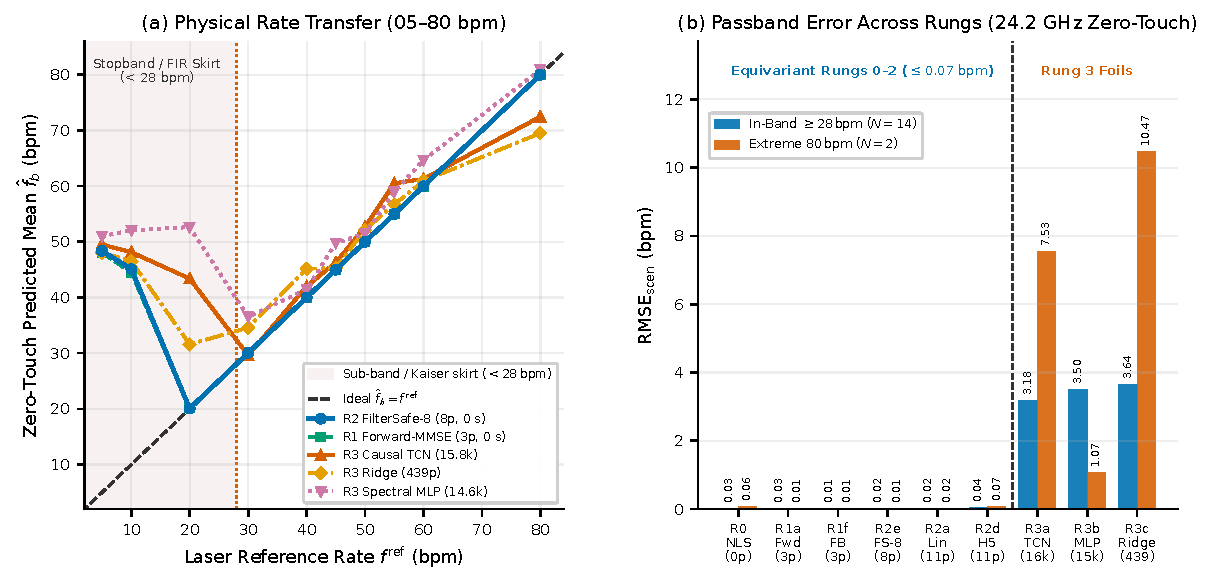
\includegraphics[width=0.95\textwidth]{stage4_external_frequency_transfer}
\caption{Zero-touch frequency transfer across the ten programmed rates and normal/deep simulator modes. Panel~(a) shows mode-averaged mean predicted rate against the laser reference relative to the locked 28~bpm reporting boundary, which separates the primary in-band results from the FIR transition skirt and below-grid stopband. Panel~(b) compares scenario-macro RMSE across Rungs~0--3 (including the R2d H5 variant) over the 14 in-band scenarios and the two 80~bpm scenarios.}
\label{fig:ch6_frequency_transfer}
\end{figure}

\section{Uncertainty and selective transfer}
\label{sec:ch6_uncertainty}

The external benchmark also tests whether Stage~3 uncertainty scores respond to simulator stopband signals and synchronization transients (Table~\ref{tab:ch6_uncertainty_transfer}). U6b retains the fixed $\tau_{\mathrm{ood}}=0.90$ cutoff and three-hop history selected in Stage~3; neither was retuned on the simulator. The stopband comparison uses steady-state windows and labels the four 5--10~bpm scenarios as out of distribution and the 14 in-band scenarios as in distribution. A separate broader comparison contrasts all six sub-band scenarios with the in-band set. These targets are deliberately distinct: success at identifying the 5--10~bpm stopband should not be read as reliable rejection across every frequency below 28~bpm.

\begin{table}[htbp]
\centering
\footnotesize
\setlength{\tabcolsep}{4pt}
\caption{Stage~4 uncertainty transfer for R2e. Risk is pooled RMSE across steady-state windows from all 20 scenarios (8,644 windows, excluding synchronization transients) at full and 80\% retention, in bpm. Stopband AUROC compares 1,731 steady-state windows at 5--10~bpm with 6,049 steady-state in-band windows; broad sub-band AUROC includes 20~bpm. Sync AUROC contrasts the 140 excluded start/end transient windows against the 6,049 steady-state in-band windows. All stopband FPR values were 0.000 at 95\% TPR.}
\label{tab:ch6_uncertainty_transfer}
\begin{tabularx}{\textwidth}{@{}>{\raggedright\arraybackslash}Xrrrr@{}}
\toprule
Proxy & RMSE ($1.0 \rightarrow 0.8$) & Stopband AUROC & Sub-band AUROC & Sync AUROC \\
\midrule
U1 posterior entropy & $17.973 \rightarrow 1.548$ & 0.9988 & 0.6679 & 0.7421 \\
U2 posterior SD & $17.973 \rightarrow 1.006$ & 0.9995 & 0.6685 & 0.7432 \\
U3 clean spectral entropy & $17.973 \rightarrow 1.014$ & 1.0000 & 0.9982 & 0.7459 \\
U4 raw spectral entropy & $17.973 \rightarrow 0.345$ & 1.0000 & 0.7484 & 0.7494 \\
U5 harmonic deficit & $17.973 \rightarrow 1.001$ & 1.0000 & 0.8552 & 0.4069 \\
U6a additive SQI & $17.973 \rightarrow 0.893$ & 1.0000 & 0.6687 & 0.7423 \\
U6b geometric SQI & $17.973 \rightarrow 0.893$ & 0.9998 & 0.6686 & 0.7422 \\
\bottomrule
\end{tabularx}
\end{table}

U6b separates the 5--10~bpm stopband from in-band simulator signals with AUROC 0.9998 and zero observed false positives at 95\% TPR; mean uncertainty is 0.0683 in-band and 0.2615 in the stopband. U2 also separates this specific stopband well (AUROC 0.9995). But discrimination falls to 0.6686 for U6b when the 20~bpm skirt is added to the out-of-band class. The composite is thus strong for the tested stopband and weak for the broader sub-band definition. It must not be described as a general frequency-boundary detector. The sync-transient AUROC is about 0.74, indicating only modest separation of those edge events.

Across steady-state windows from all 20 scenarios (8,644 windows, including stopband failures but excluding synchronization transients), the full-coverage pooled RMSE is 17.973~bpm. At 80\% retention, pooled RMSE spans 0.345~bpm for U4 to 1.548~bpm for U1, with U6a and U6b at 0.893~bpm and U2 at 1.006~bpm. This selective reduction is a descriptive result on the controlled mixture of in-band cases, stopband failures, and transients. It does not establish that a similar abstention rule would improve clinical monitoring, and the lowest-risk proxy here is not automatically appropriate for quiet-apnea handling in patient data. Figure~\ref{fig:ch6_uncertainty_conformal} summarizes this transfer and the interval results below.

\section{Conformal interval transfer}
\label{sec:ch6_conformal}

The frozen patient-calibrated C4 and C5 quantiles were applied to the primary R2e model without recalibration on simulator data. Stage~4 conformal results are reported only for R2e. The pre-freeze and post-freeze adversarial audits found that stored transfer quantiles for R1a and R2a reused the R2e quantile rather than each model's own; those fields are therefore excluded here. The full-cohort quantile uses 11 patient calibration units. At a 95\% target, its rank is $\lceil(11+1)0.95\rceil=12$, greater than the 11 available units, so the interval is vacuous; the finite-sample logic is developed in Chapter~5. The finite targets shown below are 90, 80, and 70\%.

Table~\ref{tab:ch6_conformal_transfer} reports mean full interval width, not a half-width or a value to be doubled. Coverage is summarized across simulator scenarios as the mean and minimum scenario coverage. For the 14 in-band conditions, both C4 and C5 cover every evaluated window at all three targets. The 13.27--39.08~bpm in-band widths are nevertheless broad relative to the approximately 0.02~bpm in-band RMSE; perfect observed coverage here is not evidence of a useful clinical interval or a distribution-free guarantee.

\begin{table}[htbp]
\centering
\footnotesize
\setlength{\tabcolsep}{4.5pt}
\caption{Zero-touch external conformal transfer for the frozen R2e model. Width is mean full interval width in bpm; coverage is scenario mean / minimum. The quantiles were calibrated on NICU data and not adjusted on the simulator.}
\label{tab:ch6_conformal_transfer}
\begin{tabularx}{\textwidth}{@{}>{\raggedright\arraybackslash}Xcrrrr@{}}
\toprule
Stratum & Target & C4 width & C4 coverage & C5 width & C5 coverage \\
\midrule
In-band & 90\% & 39.08 & 1.000 / 1.000 & 29.34 & 1.000 / 1.000 \\
In-band & 80\% & 26.86 & 1.000 / 1.000 & 18.02 & 1.000 / 1.000 \\
In-band & 70\% & 16.56 & 1.000 / 1.000 & 13.27 & 1.000 / 1.000 \\
\midrule
Sub-band & 90\% & 39.08 & 0.350 / 0.000 & 41.62 & 0.421 / 0.046 \\
Sub-band & 80\% & 26.86 & 0.338 / 0.000 & 25.57 & 0.360 / 0.016 \\
Sub-band & 70\% & 16.56 & 0.333 / 0.000 & 18.82 & 0.343 / 0.002 \\
\midrule
All 20 & 90\% & 39.08 & 0.805 / 0.000 & 33.03 & 0.826 / 0.046 \\
All 20 & 80\% & 26.86 & 0.801 / 0.000 & 20.29 & 0.808 / 0.016 \\
All 20 & 70\% & 16.56 & 0.800 / 0.000 & 14.93 & 0.803 / 0.002 \\
\bottomrule
\end{tabularx}
\end{table}

The high in-band coverage and low sub-band coverage reveal a strong domain boundary. At the 80\% target, C5's scenario-mean coverage is 1.000 in-band but 0.360 in the sub-band; its minimum sub-band scenario coverage is 0.016. Across all 20 scenarios, C5 reaches a scenario-mean (and pooled) coverage of 0.808, but its worst-scenario minimum is 0.016. C4 is also highly undercovered outside the in-band region. The apparently acceptable all-scenario average therefore conceals conditions in which the transferred intervals miss nearly every window. Coverage over repeated windows from a small set of simulator scenarios is descriptive and does not create independent patient-level calibration units.

\begin{figure}[htbp]
\centering
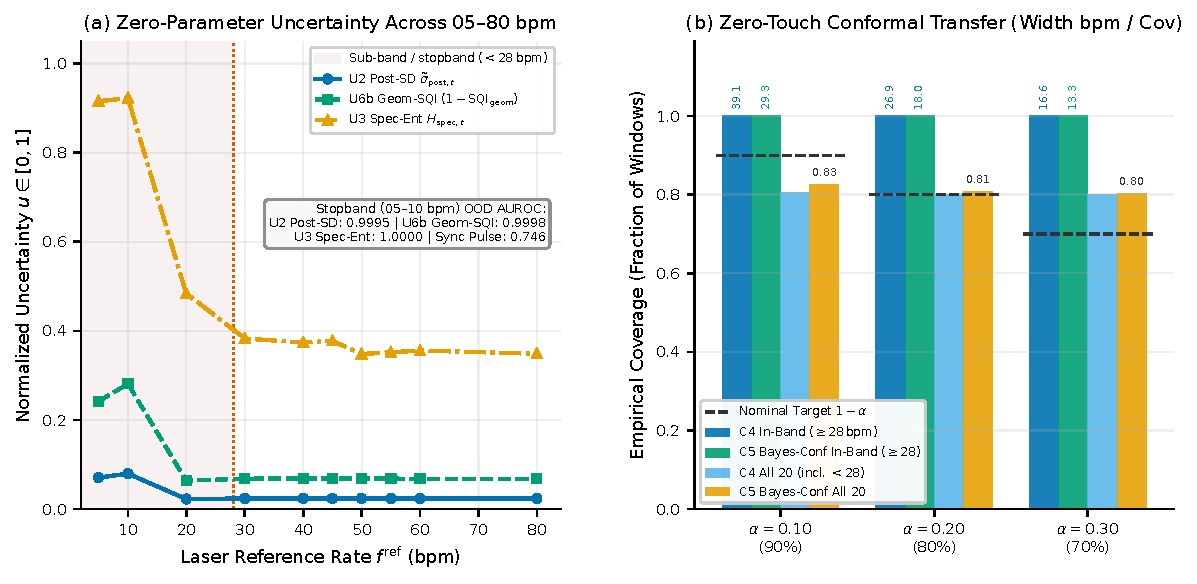
\includegraphics[width=0.95\textwidth]{stage4_external_uncertainty_and_conformal}
\caption{Stage~4 uncertainty and conformal transfer. Panel~(a) shows mode-averaged U2, U6b (zero fitted weights, locked $\tau_{\mathrm{ood}}=0.90$, and 3-hop history), and U3 scores across programmed rates, with the stopband discrimination inset and U3 synchronization-pulse AUROC (0.746). Panel~(b) compares C4 and C5 scenario-mean coverage across the 14 in-band scenarios ($\geq 28$~bpm) and all 20 scenarios, annotated with in-band mean full interval widths (sub-band breakdowns appear in Table~\ref{tab:ch6_conformal_transfer}).}
\label{fig:ch6_uncertainty_conformal}
\end{figure}

\section{Independent audit, interpretation, and limitations}

An independent clean-room audit passed all seven Stage~4 gates. It verified all 49 external source-file hashes, the disjoint 14+6 scenario partition, the laser-derived reference on independent sentinels, raw-to-16~Hz preprocessing and model outputs, stratified metrics, uncertainty and conformal results, and the serialized Gate~G5 contract. The audit confirmed the frozen archive digest given above. For the primary H0 pipeline, external $SO(2)\times\mathbb{R}_{>0}$ invariance deviations remained within $2.84\times10^{-14}$, with a quadrature-swap Nyquist residual within $2.58\times10^{-5}$~bpm; for the external H5 $O(2)\times\mathbb{R}_{>0}$ variant, the independent clean-room recomputation reported a maximum deviation of $1.42\times10^{-14}$. Sequence-level future-window perturbation tests produced exactly zero output difference for the evaluated causal sequence models and uncertainty filters (while primary H0-backed estimators still retain the fixed 3~s STFT/HPSS window lookahead). These are software and signal-processing verification results under the tested transformations, not evidence of robustness to every acquisition failure.

Taken together, Stage~4 supports three conclusions. First, the physics-constrained model family transfers with very small rate error across the simulator's in-band sinusoidal conditions, while the tested high-capacity learned models show larger calibration errors and fail at particular rate boundaries. Second, the frozen uncertainty scores identify the 5--10~bpm stopband well, but this result does not extend to the entire below-28~bpm region or to clinical artifact detection. Third, patient-derived intervals transfer empirically to the in-band simulator but under-cover substantially in the sub-band, especially at the scenario level. Each conclusion is bounded by the measured conditions and the frozen estimator pipeline.

The simulator provides controlled ground truth but only a restricted model of breathing. Its regular sinusoidal motion does not represent irregular respiratory cycles, pauses, apnea events, mixed motion, changing body position, or the noise and reference uncertainty of clinical care; the dataset authors likewise describe the simulator as covering basic functions rather than the full range of real breathing \citep{gleichauf2024time}. The study tests one external radar design at 24.2~GHz and one fixed signal-processing pipeline. Its very small in-band errors result from stable periodic signals and should not be read as expected error in an infant. The lower-frequency results show a practical limitation of the locked filter and single-channel CW measurement: below the modeled frequency range, the fundamental is attenuated or rejected and the estimate can follow a higher harmonic. The conformal results show that calibration on patient residuals does not guarantee transfer across this signal shift.

Gate~G5 therefore supports the thesis's L4 claim of zero-touch transfer to a controlled external hardware simulator. It does not authorize L5 claims of clinical superiority, bedside utility, autonomous apnea alarming, or safe use in an infant-monitoring workflow. Resolving those questions requires externally collected patient recordings, prospectively defined clinical and safety endpoints, broader hardware and site variation, and calibration cohorts large enough to support informative patient-level intervals. Chapter~7 discusses these limits and the next validation steps.
